\section{Umsetzung des Prototypen emoTrix}
Hier werden Dinge umgesetzt.
\subsection{MockUps}
\subsection{Datenerfassung in Form von Emotionstests}
\subsubsection{GSR-Test}
\subsubsectionauthor{Lukas Seemann}
Die Erfassungsmöglichkeit mit der höchsten Priorität war die Messung der Hautleitfähigkeit mithilfe von EDA- beziehungsweise GSR-Sensoren. Da dies nicht mit im Smartphone enthaltenen Sensoren möglich war, wurde zusätzlich ein Arduino-Mikrocontroller benötigt, um die Messung durchzuführen. Zunächst wird die Entwicklung auf dem Arduino-Board mit allen zusätzlichen Modulen beschrieben. Im Anschluss daran wird thematisiert, wie das Arduino-Board mit der App verbunden wurde. \newline
Für das Projekt wurde ein Arduino UNO R3 Board verwendet. \footcite[Vgl.][]{Ard18} Dieser kann mit Stromzufuhr über ein Netzteil oder per USB betrieben werden. Als Sensor wurde ein GSR Sensor des Grove-Toolkits verwendet\footcite[Vgl.][]{Gro18}, der bereits in Abbildung 5 gezeigt wird. Am Sensor selbst werden die Elektroden für die Finger angebracht. Da ein handelsübliches Arduino UNO R3 Board nicht über den benötigten Anschluss für den Grove GSR-Sensor verfügt, muss zusätzlich noch ein Grove Base Shield angebracht werden. Dieses kann auf das Arduino Board aufgesteckt werden und erweitert es um viele verschiedene Anschlüsse, unter anderem für Sensoren.
\begin{figure}[h]
	\centering
	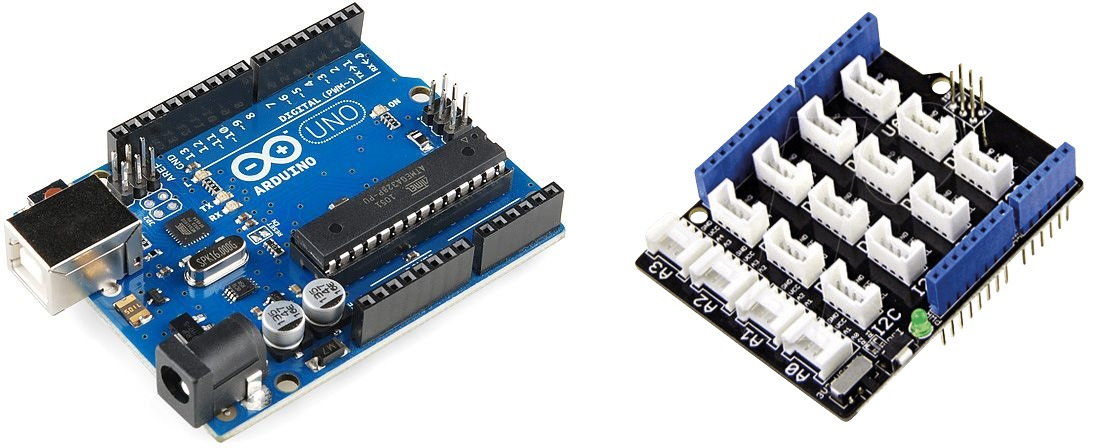
\includegraphics[width=16cm]{Bilder/arduino.jpg}
	\caption[Arduino UNO R3 (links) und Grove Base Shield]{Arduino UNO R3 (links) und Grove Base Shield\footnotemark}
\end{figure}%
\footcitetext[Bilder von:][]{Sou18, Rei18}
\newline 
Mit diesen Komponenten werden die vom Sensor zurückgelieferten Daten an den Arduino geleitet. Von dort aus müssen die Daten, an die mobile Applikation weitergeleitet werden. Aus diesem Grund muss an das Arduino Board ein Bluetooth-Modul angebracht werden, das Daten senden und empfangen kann. Das Empfangen von Daten ist notwendig, um die Messung zu Starten, wohingegen das Senden für die Übermittlung der Sensordaten benötigt wird. Heutige Smartphones verfügen meistens immer über eine Bluetooth-Schnittstelle, aus welchem Grund Bluetooth gut für die Übertragung geeignet ist. Eine weitere Möglichkeit wäre die Übertragung über WiFi gewesen. Das Arduino-Board wurde mit einem HC05-Bluetooth-Modul erweitert, welches Daten senden und empfangen kann. Dieses ist in Abbildung ? zu sehen.
\begin{figure}[h]
	\centering
	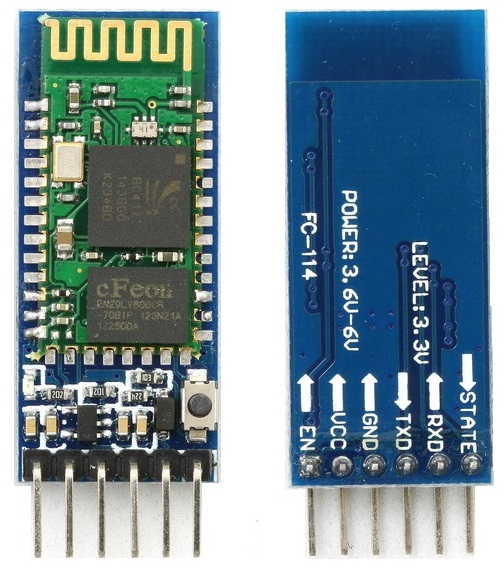
\includegraphics[width=6cm]{Bilder/hc05.jpg}
	\caption[HC-05-Bluetooth-Modul für Arduino]{HC-05-Bluetooth-Modul für Arduino\footnotemark}
\end{figure}%
\newline
Die Beschreibung der Entwicklungsarbeiten wird in zwei Teile aufgespalten. Der erste Teil ist der Quellcode des Arduinos, der zweite Teil die Entwicklung des Emotionstest in der emoTrix-App. \newline
In Listing ? ist der Quellcode des Arduinos abgebildet. In den Zeilen 1 wird die SofwareSerial-Bibliothek eingebunden, um die Kommunikation zu Modulen wie dem Bluetooth-Modul zu ermöglichen. und damit dem Arduino mitgetiel\newpage
\begin{lstlisting}[caption={Quellcode des Arduinos},style=Arduino]
#include <SoftwareSerial.h>
SoftwareSerial BTserial (10, 11); const int GSR=A0;
int sensorValue=0; int gsr_average=0;
boolean measuring = false; char BTString;

void setup(){
	BTserial.begin(9600);
}

void loop(){
	BTString = BTserial.read();
	if(BTString == 'S'){
		measuring = true;
	}
	if(BTString == 'F'){
		measuring = false;
	}
	if(measuring){
		long sum=0;
		for(int i=0;i<10;i++){ 
			sensorValue=analogRead(GSR);
			sum += sensorValue; delay(5);
		}
		gsr_average = sum/10;
		BTserial.print(gsr_average); BTserial.println( ";");
	}
}
\end{lstlisting}
\subsection{Auswertung der Testergebnisse}
\subsection{Benutzeroberfläche der App}
